\documentclass[10pt, psamsfonts]{amsart}
\usepackage[utf8]{inputenc}
\usepackage{amsfonts}
% \usepackage{hyperref}
\usepackage{amsmath}
\usepackage{xcolor}
% \usepackage{amsthm}
\usepackage{pdflscape}
\usepackage{pgfplots}
\usepackage{mathrsfs}
\usepackage{setspace}
\usepackage[margin=1in]{geometry}
\usepackage{hyperref}
\usepackage{amsthm}
\usepackage{cleveref}
\usepackage{bm}
% \usepackage[fontsize=11pt]{scrextend}

\setstretch{1.0}

\newtheorem{thm}{Theorem}[section]
\newtheorem{cor}[thm]{Corollary}
\newtheorem{prop}[thm]{Proposition}
\newtheorem{lem}[thm]{Lemma}
\newtheorem{conj}[thm]{Conjecture}
\newtheorem{quest}[thm]{Question}
\newtheorem{claim}[thm]{Claim}
\newtheorem{ppty}[thm]{Property}

\theoremstyle{definition}
\newtheorem{defn}[thm]{Definition}
\newtheorem{defns}[thm]{Definitions}
\newtheorem{con}[thm]{Construction}
\newtheorem{exmp}[thm]{Example}
\newtheorem{exmps}[thm]{Examples}
\newtheorem{notn}[thm]{Notation}
\newtheorem{notns}[thm]{Notations}
\newtheorem{addm}[thm]{Addendum}
\newtheorem{exer}[thm]{Exercise}
\newtheorem{limit}[thm]{Limitation}


\theoremstyle{remark}
\newtheorem{rem}[thm]{Remark}
\newtheorem{rems}[thm]{Remarks}
\newtheorem{warn}[thm]{Warning}
\newtheorem{sch}[thm]{Scholium}


\makeatletter
\let\c@equation\c@thm
\makeatother
\numberwithin{equation}{section}

\bibliographystyle{plain}

%--------Meta Data: Fill in your info------
\title{On Lagrangian Mechanics and the Two-Body Problem}

\author{Eric Han}

\begin{document}

\begin{abstract}
Lagrangian mechanics have long played an integral role in classical mechanics. In particular, the principles of Lagrangian mechanics have found great usage in the Two-Body Problem, allowing mathematicians and physicists to derive explicit analytic solutions to the problem for any combination of initial conditions. This paper attempts to develop a natural, mathematically rigorous understanding of the link between Lagrangian mechanics and the Two-Body Problem.
\\\\
% \noindent \textbf{Keywords.} Derivative, Differential calculus, Differentiation, Taylor's theorem, Taylor's formula, Taylor's series, Taylor's polynomial, Power function, Binomial theorem, Smooth function, Newton's interpolation formula, Finite difference, Q-derivative, Jackson derivative, Q-calculus, Quantum calculus, Q-difference, Quantum algebra\\\\
\noindent MA 562, Methods of Applied Math 2 \\
\noindent Professor Gabriel Ocker \\
\noindent Final Project\\
\noindent \textbf{Email:} ehan08@bu.edu\\
\noindent \textbf{Date:} April 26, 2024
\end{abstract}

\maketitle
\tableofcontents
\newpage

\section*{On Classical Mechanics}
For as long as humanity has existed, the study of the physical motion of projectile bodies has been of great interest. The beginnings of orbital mechanics rose with Tycho Brahe and Johann Kepler, who laid the groundwork for the study of celestial mechanics roughly 50 years before Newton's formalization of the field in his \textit{Principia}. During the plague of 1665, Newton was able to lay the groundwork for Newtonian mechanics through his laws of motion.

The study of classical mechanics can be divided into 3 central formulations:
\begin{itemize}
  \item[] \textbf{Newtonian Mechanics}, which is based on vectors in Cartesian space.
  \item[] \textbf{Lagrangian Mechanics}, which operates in a generalized coordinate space.
  \item[] \textbf{Hamiltonian Mechanics}, which operates in a phase space.
\end{itemize}
While we will unfortunately not touch on Hamiltonian mechanics, it is important for us to understand the distinction between Newtonian and Lagrangian mechanics. The first part of this paper will motivate the development of Lagrangian mechanics and tackle the derivation of the Euler-Lagrange equations and prove its equivalency to Newton's Second Law. Classical mechanics initially relied on Newtonian mechanics, but the development of the more abstract, powerful formulation of Lagrangian mechanics allow us to exploit transformational invariances and symmetries in a generalized coordinate system that are difficult to see in a standard Cartesian system using vectors.

The next part of the paper will introduce the formal statement of the Two-Body Problem and showcase the application of Lagrangian mechanics that allow us to almost magically reduce a 12-dimensional problem into a 1-dimensional problem, thereby allowing us to produce an explicit, solvable equation for the Two-Body Problem. We conclude with a brief section on the difficulty of the Three-Body Problem and its current unsolvability.
% \footnote[0]{This footnote will only appear on the draft! I basically had to teach myself the most basic fundamentals of mathematical methods for classical mechanics for this project, so please point out if any of my techniques or assumptions are faulty. I tried to do as little handwaving as possible (so with as much mathematical rigor as reasonable). However, I'm a little stuck writing about conservation of energy in the equations of motion. I'm not sure whether I should truly attempt understanding and motivating a mathematical derivation of everything or if I can just leave it as is (kind of handwavey). Additionally, the meat of the paper takes up 10-11 pages, with the appendix (incomplete) and works cited (incomplete?) providing some extra definitions and readings that I did. I hope this is a reasonable draft! I had a lot of fun writing it.}

\section{Lagrangian Mechanics}
Lagrangian mechanics is predicated, ironically, on \textit{Hamilton's} Principle of Least Action. That is, the path that a mechanical system takes is one where the path minimizes some quantity, the action, which is dependent on the body's energy as it moves. Intuitively, this means that there is some optimized motion that nature obeys, whether observing a ball's trajectory through the air or the movement of planets around one another. Remarkably, this optimal path is a fundmental result of the calculus of variations rather than a result derived from any particular physical observations.

\subsection{The Euler-Lagrange Equations}
The Euler-Lagrange equations are the beginnings of an effort to mathematically define optimized paths between an initial and terminal point in a system with constraints. Intuitively, one can view this as an optimization problem of a functional in a function space. We'll first introduce all of the definitions necessary for us to complete such an optimization problem. \cite{2}
\begin{defn}
  Let $X$ be a Banach space. A curve in $X$ is a continuous map $\gamma : [t_0, t_1] \to X$. A functional $\mathcal{F}$ is a mapping from the space of curves $\Gamma$ in $X$ to the reals. That is, $\mathcal{F}:\Gamma \to \mathbb{R}$.
\end{defn}
\begin{defn}
  Let $h = \varepsilon r$ for $0 < \varepsilon \ll 1$, $r$ some curve in $X$. A functional $\mathcal{F}$ is differentiable if $\mathcal{F}[\gamma + h] - \mathcal{F}[\gamma] = F + R$, where $F$ depends linearly on $h$ (that is, it inherits the required properties of linearity), and $R(\gamma, h) = O(h^2)$. $F(h)$ is called the differential. Note that if $\mathcal{F}$ is differentiable, its differential is uniquely defined.
\end{defn}

\begin{thm}
    \label{thm:1.3}
  Let $L$ be some functional s.t. $L:X\to \mathbb{R}$. Given a curve $\gamma$ and a small variation of the curve $h$, the functional $\mathcal{F}[\gamma] = \int_{t_0}^{t_1} L(t, x, \dot{x})$ is differentialble, and its derivaive is given by the functional
  \begin{align*}
    F(h) = \int_{t_0}^{t_1} \bigg[\frac{\partial L}{\partial x} - \frac{d}{dt} \frac{\partial L}{\partial \dot{x}}  \bigg] h dt + \bigg(\frac{\partial L}{\partial \dot{x}}h \bigg)\bigg|_{t_0}^{t_1}.
  \end{align*}
\end{thm}

\begin{proof}
\begin{align*}
      \mathcal{F}[\gamma + h] - \mathcal{F}[\gamma] & = \int_{t_0}^{t_1} [L(x+h, \dot{x} + \dot{h}, t) - L(x, \dot{x}, t)] dt\\
      & = \int_{t_0}^{t_1} \bigg[ \frac{\partial L}{\partial x} h + \frac{\partial L}{\partial \dot{x}} \dot{h} \bigg] dt + O(h^2) = F(h) + R
\end{align*}
  Integrate $\int_{t_0}^{t_1} \big[\frac{\partial L}{\partial \dot{x}} \dot{h}\big] dt$
   by parts to pull out a factor of $h$ and arrange terms accordingly.
\end{proof}

\begin{defn}
An extremal of a differential for a functional $\mathcal{F}[\gamma]$ is the minimizer or maximizer of the functional. That is, an extremal $\gamma$ is a curve s.t. $F(h) = 0$ for all $h$.
\end{defn}

We are now able to derive the titular Euler-Lagrange equations.
\begin{thm}
  The curve $\gamma: x = x(t)$ is an extremal of the functional $\mathcal{F}[\gamma] = \int_{t_0}^{t_1} L(x,\dot{x},t)dt $ on the space of curves passing through the points $x(t_0) = x_0$ and $x(t_1) = x_1$ iff
  \begin{align}
      \label{eq:Theorem 1.5}
    \frac{d}{dt} \bigg(\frac{\partial L}{\partial \dot{x}} \bigg) - \frac{\partial L}{\partial x} = 0 
  \end{align}
  along the curve $x(t)$.
\end{thm}

\noindent To prove this theorem, we need to introduce the Fundamental Lemma of the Calculus of Variations.

\begin{lem}[Fundamental Lemma of Variations]
  If a continuous function $f(t)$, $t_0\leq t \leq t_1$ satisfies $\int_{t_0}^{t_1} f(t) h(t) dt = 0$ for any continuous function $h(t)$ with $h(t_0) = h(t_1) = 0$, then f(t) must be identically 0.
\end{lem}

\begin{proof}[Proof. Fundamental Lemma of Variations]
We proceed by contradiction. Let $f(t^*) > 0$ for some $t_0 \leq t^* \leq t_1$. Since $f$ is continuous, $f(t) > c$ in some neighborhood $\Delta$ of $t^*$ s.t. $t_0 < t^* - d < t^* < t^* + d < t_1$. Let $h(t)$ be some function s.t. $h(t) > 0$ on $\Delta$, $h(t)=0$ outside $\Delta$, and $h(t) = 1$ at the midpoint of $\Delta$. It is clear, then, that $\int_{t_0}^{t_1}f(t)h(t) \geq dc > 0$. Therefore, by contradiction, $f(t^*) = 0$ for all $t^*$, $t_0 < t^* < t_1$. 
\end{proof}

\begin{proof}[Proof. Theorem 1.5]
Recall $F(h)$ from Thm. \ref{thm:1.3}.
\begin{align*}
  % \label{eq:}
  F(h) = - \int_{t_0}^{t_1} \bigg[\frac{d}{dt} \frac{\partial L}{\partial \dot{x}} -  \frac{\partial L}{\partial x} \bigg] h dt + \bigg(\frac{\partial L}{\partial \dot{x}}h \bigg)\bigg|_{t_0}^{t_1}.
\end{align*}
The term after the integral is 0 since $h(t_0) = h(t_1) = 0.$ If $\gamma$ is an extremal, then $F(h) = 0$ for all $h$ with $h(t_0) = h(t_1) = 0$. Therefore,
\begin{align*}
  \int_{t_0}^{t_1} f(t)h(t)dt = 0.
\end{align*}
where $f(t)$ is given by
\begin{align*}
  f(t) = \frac{d}{dt} \bigg(\frac{\partial L}{\partial \dot{x}}  \bigg) - \frac{\partial L}{\partial x} 
\end{align*}
for all such $h$. By the lemma, $f(t) \equiv 0$. Conversely, if $f(t) \equiv 0$, then $F(h) \equiv 0$.
\end{proof}

\begin{defn}[Euler-Lagrange Equation]
\begin{align*}
  \frac{d}{dt} \bigg(\frac{\partial L}{\partial \dot{x}}  \bigg) - \frac{\partial L}{\partial x} = 0 
\end{align*}
is called the Euler-Lagrange equation for the functional 
\begin{align*}
    \mathcal{F}[\gamma] = \int_{t_0}^{t_1}L(x, \dot{x}, t)dt.
\end{align*}
\end{defn}

Now that we've arrived at a way to determine the extrema of any given functional, we apply Hamilton's Principle of Least Action to show that the motion of any mechanical system we want to observe will be governed by its Euler-Lagrange equation.

\subsection{Newton's Second Law, and Hamilton's Principle of Least Action}
This section is written mainly from the conventions given by \cite[Arnold]{2} and \cite[Taylor]{3}.  We begin with a non-rigorous statement of Hamilton's Principle that we will build up to.
\begin{claim}
The path a mechanical system takes is one where the Euler-Lagrange equations are satisfied at every point along the path. That is, the motion of the mechanical system coincides with the extremals of a functional that models our system.
\end{claim}

\noindent To begin to understand this claim, we introduce a specific form of the functional that we used in our derivation of the Euler-Lagrange equations.

\begin{defn}
The \textbf{Lagrangian} of a system, $\mathfrak{L}$, is the difference between the kinetic energy $T$ and potential energy $V$ of the system, $\mathfrak{L} = T - V$.
\end{defn}
\begin{defn}
The action of a system, S, is the integral of the Lagrangian over a finite time interval, the initial and terminal time.
\begin{align*}
  S[u] = \int_{t_0}^{t_1} \mathfrak{L}\,dt  
\end{align*}
\end{defn}

Recall that for a system of particles with conservative forces defined via the gradient of a potential, Newton's Second Law for a vector force $\textbf{F}$ holds:
\begin{align}
  \label{eq:Newton's Second}
  \bm{F}_i = m \ddot{x}_i.
\end{align}
For a mechanical system, the kinetic and potential energies can be expressed as 
\begin{align}
  \label{eq:Kinetic, Potential}
  V = V(x) \text{ and } T = \frac{1}{2} \sum_i m_i \dot{x}_i^2
\end{align}
The right-hand side of Newton's Second Law (\ref{eq:Newton's Second}) is the derivative of momentum, which can be defined as the derivative of kinetic energy with respect to velocity,
\begin{align}
\label{eq:kinetic}
  \frac{\partial T }{\partial \dot{x}_i} = m\ddot{x}_i = \bm{p}_i.
\end{align}
The left-hand side of (\ref{eq:Newton's Second}) is the negative derivative of potential energy with respect to position,
\begin{align}
  \label{eq:potential}
  -\frac{\partial V}{\partial x} = \bm{F}_i.
 \end{align}
Our goal then, is to demonstrate that Newton's Second Law produces an extremal for the Lagrangian - that is, it satisfies the Euler Lagrange equation at all points.

\begin{thm}[Hamilton's Principle of Least Action]
Motion of any mechanical system obeying Newton's Second Law associated with a Lagrangian $\mathfrak{L}$ coincides with the extremals of the functional
\begin{align*}
  \Phi[\gamma] = \int_{t_0}^{t_1} \mathfrak{L}  (x, \dot{x}, t)dt.
\end{align*}
\end{thm}

\begin{proof}
By Theorem 1.5, any curve that is an extremal of a functional is identical to a curve where the Euler-Lagrange equation is satisfied everywhere. We will show that a trajectory obeying Newton's Second Law, $\textbf{F}_{i} = m\ddot{x}_i$, satisfies the Euler-Lagrange at all points. Utilizing our earlier definitions of force in terms of kinetic and potential energy, given by (\ref{eq:Kinetic, Potential}), the Lagrangian of our system can be defined as
\begin{align}
  \label{eq:Lagrangian KP}
  \mathfrak{L} = \frac{1}{2} \sum_i m_i \dot{x}_i^2 - V(x).
\end{align}
We first plug in our Lagrangian (\ref{eq:Lagrangian KP}) into the Euler-Lagrange equations,
\begin{align*}
  % \label{eq:}
  \frac{\partial \mathfrak{L}}{\partial x} - \frac{d}{dt} \frac{\partial \mathfrak{L}}{\partial \dot{x}} &= -\frac{\partial V}{\partial x} - \frac{d}{dt} \frac{\partial T}{\partial \dot{x}_i}.
\end{align*}
Then, we use the equivalencies we established earlier in (\ref{eq:kinetic}) and (\ref{eq:potential}), giving us
\begin{align*}
  % \label{eq:}
  -\frac{\partial V}{\partial x} - \frac{d}{dt} \frac{\partial T}{\partial \dot{x}_i} &= \bm{F}_i - m\ddot{x}_i \\
  &= \bm{F}_i - \bm{F}_i = 0.
\end{align*}
Because plugging in $\mathfrak{L}$ into the Euler-Lagrange equations returns 0, this implies that Newton's Second Law is an extremum of $\Phi$. Conversely, one can do the exact procedure in reverse to show that an extremum of $\Phi$ can imply Newton's Second Law.
\end{proof}

Through this, we have proved the following three statements equivalent for mechanical systems:
\begin{enumerate}
\item The optimal path is determined by the Euler-Lagrange equation.
\item The same optimal path is determined by Newton's Second Law.
\item The same optimal path is determined by Hamilton's Principle of Least Action.
\end{enumerate}
The second statement is of particular use to us, as we may now transition from the Cartesian coordinates of Newtonian Mechanics to the generalized coordinate space of Lagrangian mechanics.

\subsection{Generalized Coordinates and Invariance}
In a characteristic move for physicists and mathematicians, we attempt to generalize mechanics in Cartesian space (which utilizes vectors) to a generalized coordinate space where we may use scalar representations of motion, such as kinetic and potential energy. 
However, unlike physicists and more akin to mathematicians, we will try to rely as little as possible on physical assumptions, and to try and derive most things through techniques of the calculus of variations.

The Lagrangian formulation of classical mechanics has two central advantages over the Newtonian formulation. First, Lagrange's equations take the same form in any coordinate system, as coordinate transforms are as easy as defining a function that transforms each coordinate in your system. Second, the Lagrangian approach eliminates forces of constraints, such as a particle forced to move on a curved surface. We will be exploiting the first of these two properties in this section. \cite[Arnold]{2}

We must first define our generalized coordinate system.
\begin{defns}
\;
\begin{itemize}
\item[] \textbf{Generalized Coordinates}: $\{q_1, q_2, ..., q_i,...,q_N\}$
\item[] \textbf{Generalized Velocities}: $\{\dot{q}_1, \dot{q}_2, ..., \dot{q}_i,...\dot{q}_N\}$
\item[] \textbf{Generalized Force}: $\cfrac{\partial \mathfrak{L}}{\partial q_i} $
\item[] \textbf{Generalized Momentum}: $\cfrac{\partial \mathfrak{L}}{\partial \dot{q}_i}$
\end{itemize}
\end{defns}
\noindent We assume that our generalized coordinates parametrize all of our configuration space, so that each point can be described by $\{q_j\}$ or $\{x_i\}$ where $i, j \in [1, N]$. Each set of coordinates can be thought of as a function of the other and time:
\begin{align*}
  % \label{eq:}
  q_j &= q_j(x_1,...,x_N; t)\\
  x_i &= x_i(q_1,...,q_N; t).
\end{align*}
We may use our new generalized coordinates in the Lagrangian.

\begin{defn}
Let $\mathfrak{L}[x, \dot{x}, t]$ be a Lagrangian in a Cartesian space. Then, 
\begin{align*}
  % \label{eq:}
  \tilde{\mathfrak{L}}[q, \dot{q}, t] = \mathfrak{L}[x(q,t), \dot{x}(q, \dot{q}, t)] 
\end{align*}
is the Lagrangian in a generalized coordinate space. 
\end{defn}

Before continuing any further, it's important to understand our final goal for generalizing Newtonian mechanics into the Lagrangian framework.
\begin{claim}
  The Euler-Lagrange equations in Cartesian space and the Euler-Lagrange equations in generalized coordinate space agree at corresponding physical points in space.
\end{claim}
We would like to show that the optimal trajectory taken by a mass obeying Newton's Second Law remains the "same" under coordinate transformation so that we may move into the generalized coordinate space of Lagrangian mechanics. That is, the Euler-Lagrange equations are invariant to coordinate transforms.

\begin{defn}
Consider a family of transformations of $\mathbb{R}^d$, $h_s(q):\mathbb{R}^d \to \mathbb{R}^d $, where $s \in \mathbb{R}$, and $h_s(q)$ is continuous in both $q$ and $s$, and $h_0(q) = q$. A functional $\mathcal{F}[q, \dot{q}, t]$ is invariant under the action of the family of transformations of $\mathbb{R}^d$, $h_s(q): \mathbb{R}^n \to \mathbb{R}^d$, if $\mathcal{F}$ does not change when $q(t)$ is replaced by the transform $h_s(q(t))$. That is, for any function $q(t)$,
\begin{align*}
  % \label{eq:}
  \mathcal{F}[h_s(q(t)), \frac{d}{dt} h_s(q(t))] = \mathcal{F}[q(t), \frac{d}{dt} q(t)].
\end{align*}
\cite[Chertkov, Clark]{7}
\end{defn}

% \begin{thm}[Noether's Theorem]
% If the Lagrangian $\mathfrak{L}$ is invariant under the action of a one-parameter family of transformations, $h_s(u(t))$, then the quantity
% \begin{align*}
%   % \label{eq:}
%   I(q, \dot{q}) \equiv \mathfrak{L}_{\dot{q}} \cdot \frac{d}{ds} h_s(q) \bigg|_{s=0}
% \end{align*}
% is constant along any solution of the Euler-Lagrange equation. This quantity is called the integral of motion.
% \end{thm}
% \noindent The details of the proof for this theorem are left to Chertkov and Clark. \\

Invariance under coordinate transformation lets us choose a coordinate system that is convenient for us, as the trajectory of the mass is unchanged, regardless of the coordinate system we use. Our aim then, is to prove that the Euler-Lagrange equations are invariant under coordinate transformations.

\begin{defn}
Let $q_j$ denote position in generalized coordinates. Then velocity is defined as
\begin{align}
  \label{eq:Formal Velocity}
  \dot{q}_j = \sum_i \frac{\partial q_j}{\partial x_i} \dot{x}_i + \frac{\partial q_j}{\partial t}. 
\end{align}
\end{defn}
\noindent It follows that
\begin{align}
  \label{eq:Proportionality}
  \frac{\partial \dot{q}_j}{\partial \dot{x}_i} = \frac{\partial q_j}{\partial x_i}.
\end{align}
That is, observing the movement of particles in a system, the change in position over time across different coordinate spaces is proportional to their changes in position.\\

Additionally, it would be wise to first define the total time derivative for a function, as we must use it in the proof for Theorem \ref{thm: Invariance of EL}.
\begin{defn}
    \label{def:Time Deriv Def}
% \footnote{I may move this definition to the beginning of the section as \ref{eq:Formal Velocity} is a direct consequence of this.}
For any function $f(x,t)$ in a configuration space\footnote{See (\ref{def: Configuration Space}) in the appendix}, the total time derivative is
\begin{align}
  \label{eq:Time Derivative}
  \frac{df}{dt} = \sum_j \frac{\partial f}{\partial x_j} \dot{x}_j + \frac{\partial f}{\partial t}. 
\end{align}
\end{defn}

\begin{thm}
    \label{thm: Invariance of EL}
  The Euler-Lagrange equations are invariant to coordinate transformations. In generalized coordinate space, it produces an Euler-Lagrange equation of the form
  \begin{align*}
    % \label{eq:}
    \frac{d}{dt} \bigg( \frac{\partial \mathfrak{L}}{\partial \dot{q}_j}  \bigg) - \frac{\partial \mathfrak{L} }{\partial q_j} = 0.
  \end{align*}
\end{thm}

\begin{proof}
The chain rule tells us that
\begin{align}
  \label{eq:Chain Rule Lagrangian xdot} 
  % \setcounter{equation}{19}
  \frac{\partial L}{\partial \dot{x}_i}  = \sum_k \frac{\partial L}{\partial q_k} \frac{\partial q_k}{\partial \dot{x}_i} + \frac{\partial L}{\partial \dot{q}_k} \frac{\partial \dot{q}_k}{\partial \dot{x}_j}.
\end{align}
Recall that $q_k$ denotes position in our generalized coordinates. Thus, the first term disappears because $q_k$ is dependent on position and time, $x_k$ and $t$, but not on the velocity in Cartesian coordinates $\dot{x}_k$. From (\ref{eq:Proportionality}), we may rewrite (\ref{eq:Chain Rule Lagrangian xdot}) as
\begin{align*}
  % \label{eq:}
  \frac{\partial L}{\partial \dot{x}_i} = \sum_j \frac{\partial L}{\partial \dot{q}_j} \frac{\partial q_j}{\partial x_i}. 
\end{align*}
The Euler-Lagrange equation demands that we take the time derivative of this function. We don't want a partial derivative, which holds the point in configuration space fixed, but rather the \textit{total} time derivative, which is the derivative along the path that the system takes as it moves through configuration spaces.

\noindent Referring to Definition \ref{def:Time Deriv Def}, using the product rule and then applying (\ref{eq:Time Derivative}) to the second term after the product rule, the time derivative of $\partial L/\partial \dot{x}_i$ is
\begin{align}
  \label{eq:Time Derivative Lagrangian}
  \sum_j \bigg(\frac{d}{dt} \frac{\partial L}{\partial \dot{q}_j}  \bigg) \frac{\partial q_j}{\partial x_i} + \sum_j \frac{\partial L}{\partial \dot{q}_j} \bigg(\sum_{k} \frac{\partial^2 q_j}{\partial x_i \partial x_k} \dot{x}_k + \frac{\partial^2 q_j}{\partial x_i \partial t}  \bigg).
\end{align}

Also, by the chain rule, 
\begin{align*}
  % \label{eq:}
  \frac{\partial L}{\partial x_i}  = \sum_j \frac{\partial L}{\partial q_j} \frac{\partial q_j}{\partial x_i} + \sum_j \frac{\partial L}{\partial \dot{q}_j} \frac{\partial \dot{q}_j}{\partial x_i}.
\end{align*}
The last term no longer vanishes, as $\dot{q}_j$ generally depends on both position and velocity. From (\ref{eq:Formal Velocity}), 
\begin{gather*}
  \frac{\partial \dot{q}_j}{\partial x_i} = \sum_k \frac{\partial^2 q_j}{\partial x_i \partial x_k} \dot{x}_k + \frac{\partial^2 q_j}{\partial x_i \partial t},
\end{gather*}
so
\begin{gather}
\label{eq:Spatial Lagrangian}
  \frac{\partial L}{\partial x_i} = \sum_j \frac{\partial L}{\partial q_j} \frac{\partial q_j}{\partial x_i} + \sum_j \frac{\partial L}{\partial \dot{q}_j}\bigg(\sum_k \frac{\partial^2 q_j}{\partial x_i \partial x_k} \dot{x}_k + \frac{\partial^2 q_j}{\partial x_i \partial t}  \bigg).
\end{gather}
The Euler-Lagrange equation says that \ref{eq:Time Derivative Lagrangian} and \ref{eq:Spatial Lagrangian} are equal, and in subtracting them, the second terms cancel. We are left with
\begin{align*}
  % \label{eq:}
  0 = \sum_j \bigg(\frac{d}{dt} \frac{\partial L}{\partial \dot{q}_j} - \frac{\partial L}{\partial q_j} \bigg) \frac{\partial q_j}{\partial x_i} .
\end{align*}

The matrix operator provided by $\partial q_j/\partial x_i $ is nonsingular, and thus has a trivial nullspace. Therefore, the only way for this quantity to be 0 is for
\begin{align*}
  % \label{eq:}
  \frac{d}{dt} \frac{\partial L}{\partial \dot{q}_j} - \frac{\partial L}{\partial q_j} = 0
\end{align*}

We have thus derived the Euler-Lagrange equations in generalized coordinates, and proved that they are invariant to coordinate transformation because the form of the Euler-Lagrange equations are the same.\footnote{This proof is somewhat unwieldy due to the tedious algebra one must slog their way through in applying (\ref{eq:Time Derivative}). However, the advantage of this proof is that it provides an explicit, closed form for the derivatives we use in our calculations.  I also really don't want to typeset the new proof. For a far more elegant proof using a non-explicit time derivative, reference \cite{6} David Morin's Classical Mechanics, Chapter 6.4.}
\end{proof}
A very beautiful result about the symmetries of the Lagrangian $\mathfrak{L}$ itself can be found in \cite{6}.\\

This is the central result that we have been aiming for. We began by attempting to discern the most efficient path for a system with constraints which we modeled as an optimization problem in a Banach space. We arrived at the Euler-Lagrange equations for an arbitrary functional, which gave us the extrema of the functional. We then extended this notion to the realm of classical mechanics by introducing Hamilton's Principle of Least Action and proving it equivalent to both Newton's Second Law of Motion and the Euler-Lagrange equations, showing that the most optimized paths of motion for mechanical systems were those which satisfied the Euler-Lagrange equations. Finally, we showed that the Euler-Lagrange equations are invariant under coordinate transformations, allowing us to adopt a more abstract formalization of mechanics in Langrangian mechanics. Now, we may approach the Two-Body Problem with these tools in hand.

\section{The Two-Body Problem}
The Two-Body Problem is one of the most fundamental problems in the field of classical mechanics. It was first tackled by Newton in his \textit{Principia} using geometric arguments and his Universal Law of Gravitation. Broadly, the problem deals with an isolated system of two bodies. We assume that the only forces in the system are those of the two bodies acting upon one another. There are several examples of this problem that naturally arise in our universe: the moon and the Earth, the Earth and the Sun, or a binary system of two stars. Realistically, we cannot exclude even the ``small'' perturbative forces that these systems experience, but the reduction of the problem will still provide a good first approximation of such systems. The following sections are primarily written with the conventions of \cite[Morin]{6} and \cite[Taylor]{7}.

\subsection{Applying the Euler-Lagrange Equations}
Consider two bodies in space with masses $m_1, m_2$ at positions $\bm{r}_1, \bm{r}_2$ in space. The size of the bodies is irrelevant in that they are separated so greatly in magnitude that irrespective of their actual size, they may be represented by point masses in space. The only forces present in the system are the force of body 1 on body 2 and vice versa, $\bm{F}_{12} $ and $\bm{F}_{21}$. \\
% We assume these are conservative forces and can thus be regarded as gradients of the potential, $U(\bm{r}_1, \bm{r}_2)$.\\ Maybe I'll include this? I want to talk about conservative forces later.

To describe $n$ bodies in standard Euclidean 3-space, one normally needs a $6n$-dimensional configuration space. 3 exist to denote position, and 3 exist for momentum. For the Two-Body Problem, one would need 12 separate equations describing each parameter over time. However, because of the Euler-Lagrange equations we've derived, we may attempt to reduce the problem to a one-dimensional problem by exploiting transformational invariances in the Lagrangian.

\begin{defn}
  For any isolated system where the only forces in the system are those of the particles acting upon one another, the system must be \textbf{translationally invariant}. That is, if we bodily translate the system to a new position without changing the relative positions of the particles, the interparticle forces should stay the same.
\end{defn}

First, we would like to state our scalar quantities of energy for the problem. Here, $U(\bm{r}_1, \bm{r}_2)$ is the potential of an isolated system, so it is translationally invariant. Thus, it depends exclusively on the position of the objects relative to each other, $U(\bm{r}_1, \bm{r}_2) = U(|\bm{r}_1 - \bm{r}_2|) $. Exploiting the translational invariance of the system, we thus define a new variable,
\begin{align*}
  % \label{eq:}
  \bm{r} = |\bm{r}_1 - \bm{r}_2|.
\end{align*}
We refer to $r$ as the magnitude of the relative position $\bm{r}$. With this definition, we can also restate our definition of potential energy to depend exclusively on $r$,
\begin{align*}
  % \label{eq:}
  U = U(r).
\end{align*}
Recall that kinetic energy is defined 
\begin{align*}
  % \label{eq:}
  T &= \frac{1}{2} \sum_i  m_i \dot{x}_i^2 \\
    &= \frac{1}{2} (m_1 \dot{\bm{r}_1}^2 + m_2 \dot{\bm{r}_2}^2).
\end{align*}

We may now frame our problem mathematically. We would like to find the possible motions of two bodies that obey the Lagrangian
\begin{gather*}
      % \label{eq:}
  \mathfrak{L} = \frac{1}{2} (m_1 \bm{r}_1^2 + m_2 \bm{r}_2^2) - U(r).
\end{gather*}
To do this, we will do as we've been doing - Hamilton's principle frames Newton's Second Law as an optimization problem involving the Lagrangian $\mathfrak{L}$. This produces the Euler-Lagrange equations, which will tell us the trajectory that the bodies must obey in their paths through space.

\subsection{Generalizing Coordinate Space} To make working with the Lagrangian
easier, we would like to adopt a generalized coordinate space. We have already
reduced the three-dimensional notion of position to one-dimensional relative
position, $\bm{r}$. The question we ask then, is how to represent the similarly
three-dimensional momentum. 

The first step is to take advantage of the fact that the rotation of our system typically takes place around the center of mass. This is given explicitly by
\begin{align*}
  % \label{eq:}
  \bm{R} = \frac{m_1 \bm{r}_1 + m_2 \bm{r}_2}{M},
\end{align*}
where $M = m_1 + m_2$, the total mass.
% Additionally, we will take it as given that the total momentum of two bodies can be expressed as
% \begin{align*}
%   % \label{eq:}
%   \bm{P} = M\dot{{R}}.
% \end{align*}
% We know that momentum is a conserved quantity, that is, it remains constant in a system. Therefore, $\dot{\bm{R}} $ must be constant as well. This will play a large role in 

\noindent Now, $\bm{r}_1$ and $\bm{r}_2$ can be expressed entirely through their relative position and the system's center of mass
\begin{align*}
  % \label{eq:}
  \bm{r}_1 &= \bm{R} + \frac{m_2}{M} \bm{r} \\
  \bm{r}_2 &= \bm{R} - \frac{m_1}{M} \bm{r}.
\end{align*}
\noindent We can now express kinetic energy as
\begin{align*}
  % \label{eq:}
  T & = \frac{1}{2} (m_1 \dot{\bm{r}_1}^2 + m_2 \dot{\bm{r}_2}^2) \\
    & = \frac{1}{2} \bigg(m_1 \bigg(\dot{\bm{R}}+\frac{m_2}{M} \dot{\bm{r}}\bigg)^2 + m_2 \bigg(\dot{\bm{R}} - \frac{m_1}{M} \dot{\bm{r}} \bigg)^2 \bigg)\\
    & = \frac{1}{2} \bigg( M \dot{\bm{R}}^2 + \mu\dot{\bm{r}}^2 \bigg),
\end{align*}
where $\mu = \frac{m_1 m_2}{M} \text{, the reduced mass} $.
We have thus arrived at a configuration space with 4 degrees of freedom for two bodies \cite{3}.\\

Now, the remarkability of the invariance of the Euler-Lagrange equations, presents itself. We may write the Lagrangian
\begin{align}
  \label{eq:TB Lagrangian}
  \mathfrak{L} &= T - U \notag \\
               &= \frac{1}{2} M \dot{\bm{R}}^2 + \frac{1}{2} \mu\dot{\bm{r}}^2 - U(r). 
\end{align}
The Lagrangian can then be split into two separate pieces, with one piece dependent exclusively on the center of mass $\bm{R}$ and the other dependent exclusively on $\bm{r}$. We can then solve for the motions of $\bm{R}$ and $\bm{r}$ separately, but it will turn out that even this isn't necessary!

\subsection{Conserved Quantities and Further Reduction}
Consider the case where the Lagrangian $\mathfrak{L}$ doesn't depend on position ${q_k}$. Then,
\begin{align*}
  % \label{eq:}
  \frac{d}{dt} \bigg(\frac{\partial \mathfrak{L}}{\partial \dot{q}_k}  \bigg) - \frac{\partial \mathfrak{L}}{\partial q_k} = 0 \Rightarrow \frac{\partial \mathfrak{L}}{\partial \dot{q}_k} = C,  
\end{align*}
where $C$ is a time-independent constant (although a time-dependent constant wouldn't be much of a constant at all).
\begin{defn}
  A coordinate that doesn't explicitly appear in the Lagrangian is called a \textbf{cyclic coordinate}. If a quantity of a mechanical system remains constant over time, it is a \textbf{conserved quantity}.
\end{defn}

\noindent So, in our Lagrangian, ${\partial \mathfrak{L}}/{\partial \dot{q}_k}$ is a conserved quantity. In Cartesian coordinates, we would consider the momentum $\bm{p} = {\partial \mathfrak{L}}/{\partial \dot{x}_k}$ a conserved quantity, which reassuringly correlates with physics. 

\begin{defn}
For the Lagrangian in generalized coordinates,
  $\cfrac{\partial \mathfrak{L}}{\partial \dot{q}_k}$
is the generalized momentum. If this quantity is constant over time, we call it a conserved momentum.
\end{defn}

Recall the Lagrangian of the Two-Body Problem. We know that $\bm{R}$ is the position of the center of mass in our Lagrangian, and (\ref{eq:TB Lagrangian}) is independent of $\bm{R}$, so we know that generalized momentum, $\dot{\bm{R}}$, must be a conserved quantity. If generalized momentum is constant, then naturally, the generalized velocity must be constant as well. Thus, the center of mass of our system $\bm{R}$ moves with constant velocity. The problem then reduces itself if we choose a clever frame of reference: because $\bm{R}$ is constant, choosing an inertial frame of reference where the center of mass is stationary and the total momentum is zero allows us to ignore the term dependent on $\bm{R}$ in the Lagrangian entirely!

We are left to observe the behavior of the Lagrangian
\begin{align}
  \label{eq:One Param Lag}
  \mathfrak{L} = \frac{1}{2} \mu \dot{\bm{r}}^2 - U(r).
\end{align}
Solving for the Euler-Lagrange equation, we get
\begin{gather}
  \label{eq:One Param EL}
  \mu \ddot{\bm{r}} + \nabla U(\bm{r}) = 0 \notag \\
  \mu \ddot{\bm{r}} = -\nabla U(\bm{r})
\end{gather}
\noindent So, all that's left to solve is this equation, governing a single particle with mass $\mu$, position $\bm{r}$, and potential $U$.

Taking the center of mass as the origin of our system, $\bm{r}(t)$ tells us the motion of either particle relative to the center of mass. Inherent in this observation lies another opportunity to simplify our problem. Namely, we would like to show that as a consequence of the conservation of angular momentum, the movement of the two bodies takes place in a plane, reducing our problem to 2 dimensions.

In any frame of reference, the total angular momentum is given by
\begin{align}
  \label{eq: Angular Momentum General Frame}
  \bm{L} & = \bm{r}_1 \times \bm{p}_1 + \bm{r}_2 \times \bm{p}_2 \notag \\
         & = m_1 \bm{r}_1 \times \dot{\bm{r}}_1 + m_2 \bm{r}_2 \times \dot{\bm{r}}_2.
\end{align}
In the frame of reference we've chosen where $\bm{R} = 0$, the positions of the particles are given by
\begin{align*}
  % \label{eq:}
  \bm{r}_1 &= \frac{m_2}{M} \bm{r}\\
  \bm{r}_2 &= -\frac{m_1}{M} \bm{r}.
\end{align*}
\noindent So, our angular momentum given in the CM frame of reference is
\begin{align}
  \label{eq:Angular Momentum CM Frame}
  \bm{L} &= \frac{m_1 m_2}{M^2} (m_2 \bm{r} \times \dot{\bm{r}} + m_1 \bm{r} \times \dot{\bm{r}}) \notag \\
         &= \bm{r} \times \mu \dot{\bm{r}}
\end{align}
where $\mu$ is the reduced mass. Because angular momentum is conserved, the vector, and more importantly, the direction of the vector $\bm{r} \times \dot{\bm{r}}$ is constant. This implies that the two vectors $\bm{r}$ and $\dot{\bm{r}}$ remain in a fixed plane. We've thus reduced the problem to a two-dimensional problem!

Here arises a few barriers in our current statement of the problem. First, we must remember that our problem is not a purely mathematical one. The ultimate goal is to be able to accurately predict the motion of two bodies in a mechanical system, so we may want to choose a more suitable coordinate system now that we've done all the reductions we can in a general coordinate space. Second, there exists a restriction on the Lagrangian in that the potential depends only on the magnitude $r$ of $\bm{r}$. Fortunately, polar coordinates remedy both these problems surprisingly elegantly and also send us on our way to deriving Kepler's laws of planetary motion.

\subsection{Polar Coordinates, Equations of Motion, and Reduction to a One-Dimensional Problem} We will utilize polar coordinates in $r$ and $\theta$ to parametrize our Lagrangian, taking advantage of its invariance under coordinate transformation once again. This gives us, from (\ref{eq:One Param Lag}),
\begin{align*}
  % \label{eq:}
  \mathfrak{L} = \frac{1}{2} \mu (\dot{r}^2 +\dot{r}^2 \dot{\theta}^2) - U(r).
\end{align*}
Notice the Lagrangian is independent of $\theta$. It is thus a cyclic coordinate. The Euler-Lagrange equation corresponding to $\theta$ is then
\begin{align}
  \label{eq: Theta Eq}
  \frac{\partial \mathfrak{L}}{\partial \dot{\theta}} = \mu r^2 \dot{\theta} = C = l,
\end{align}
where $C$ is a constant and $l$ denotes the angular momentum of the Lagrangian.
\begin{defn}
The angular momentum in polar coordinates is defined $m r^2 \omega$ where $\omega$ denotes angle, $m$ denotes mass, and $r$ denotes position.
\end{defn}
It is obvious then, that the Euler-Lagrange equation corresponding to $\theta$ is simply a restatement of the conservation of angular momentum \cite{3}.

More interestingly, the Euler-Lagrange equation corresponding to $r$ can be computed to be
\begin{align}
  \label{eq: Radial Eq}
  &\frac{\partial \mathfrak{L}}{\partial r} = \frac{d}{dt} \frac{\partial \mathfrak{L}}{\partial \dot{r}} \notag \\
  \Rightarrow\quad& \mu r \dot{\theta}^2 - \frac{dU}{dr} = \mu \ddot{r}.
\end{align}
Somewhat remarkably, Newton's Second Law manifests in this equation as well. Moving the $\mu r \dot{\theta}^2$ to the right side will give you
\begin{align*}
  % \label{eq:}
  - \frac{dU}{dr} &= \mu \ddot{r} - \mu r \dot{\theta}^2
  % 
\end{align*}
which is the radial component of $\bm{F} = \mu \bm{a}$.

We thus arrive at 2 equations of motion that we have to solve. One is given in terms of $\theta$ (\ref{eq: Theta Eq}) and the other in terms of $r$ (\ref{eq: Radial Eq}). The angular momentum, given by $l$, is determined by the initial conditions of our system and is a constant. Therefore, it would be nice if we could express $\dot{\theta}$ in terms of $l$. Conveniently, with (\ref{eq: Theta Eq}), we can do exactly this.
\begin{align}
  \label{eq:Angular Momentum in l}
  \dot{\theta} = \frac{l}{\mu r^2} 
\end{align}
From here,
(\ref{eq: Radial Eq}) can be rewritten as 
\begin{align*}
  \label{eq:}
  \mu \ddot{r} = -\frac{dU}{dr} + F_{CF}
\end{align*}
where $F_{CF} = \mu r \dot{\theta}^2$ is an outward centrifugal force. We can then rewrite $F_{CF}$ in terms of the constant $l$,
\begin{gather*}
  F_{CF} = \mu r \dot{\theta}^2 = \frac{l^2}{\mu r^3},
\end{gather*}
which allows us to define the centrifugal force in terms of a centrifugal potential energy 
\begin{gather}
    \label{eq:centrifugal potential}
  F_{CF} = -\frac{d}{dr} \bigg(\frac{l^2}{2\mu r^2}  \bigg) =  -\frac{dU_{CF}}{dr} \notag\\
  U_{CF}(r) = \frac{l^2}{2\mu r^2} 
\end{gather}

This is particularly helpful, as we may now rewrite ($\ref{eq: Radial Eq}$) in terms of effective potential energy,
\begin{defn}
  In it's most basic form, the effective potential energy of a system is defined as the sum of the actual potential energy $U(r)$ with the centrifugal potential energy $U_{CF}(r)$.
\end{defn}
So, 
\begin{align}
  \label{eq:Final Result}
  \mu \ddot{r} = -\frac{d}{dr} U_{\text{eff}}(r).
\end{align}
where $U_{\text{eff}}(r)$ is expressed as
\begin{align}
  \label{eq: Effective Potential}
  U_{\text{eff}}(r) = U(r) + U_{CF}(r) = U(r) + \frac{l^2}{2\mu r^2}. 
\end{align}

We are almost done. The details of the orbit will be explicitly given by looking more closely at (\ref{eq:Final Result}). Multiplying both sides of the equation by $\dot{r}$, we get\footnote{Some real abuse of Leibnitz notation going on here.}
\begin{align*}
  & \frac{d}{dt} \bigg(\frac{1}{2} \mu \dot{r}^2 \bigg) = -\frac{d}{dt} U_{\text{eff}}(r)\\
  \Rightarrow \quad &  \frac{1}{2} \mu \dot{r}^2 + U_{\text{eff}}(r) = \text{const.}
\end{align*}
This result demonstrates the conservation of energy within our system. Expanding $U_{\text{eff}}(r) $ explicity as given in (\ref{eq: Effective Potential}),
\begin{gather}
    \label{eq:Energy Conservation}
  \frac{1}{2} \mu \dot{r}^2 + U_{\text{eff}}(r) = \frac{1}{2}  \mu \dot{r}^2 + \frac{1}{2} \mu r^2 \dot{\theta} ^2 + U(r)
  = E.
\end{gather}

Finally, we arrive at a complete picture of our desired result. By (\ref{eq:Final Result}), the radial motion of the particle is exactly the same as if the particle were moving in a single dimension with an effective potential. We have thus reduced the original, intimidating, 12-dimensional form of the Two-Body Problem to a single-dimensional problem which can be solved numerically or analytically with many sets of initial conditions. The radial motion of the particle is exactly identical to the movement of the particle moving in one-dimension with an effective potential energy. 

Additionally, by (\ref{eq:Energy Conservation}), the total energy is representable as the sum of the one-dimensional kinetic energy of the radial motion and the effective potential energy, both of which have explicit forms.

From here, one may go on to determine Kepler's Laws and make many other physical observations of the motions of celestial bodies. The most amazing part of this is that through the methods of the calculus of variations, we were able to discern a profoundly physical interaction in classical mechanics.\\

To demonstrate the power of our reduction of the Two-Body Problem, we can use the \textit{Kepler Problem}, named after Johannes Kepler, who first derived the mathematical motions of the planets. This example comes from \cite[Taylor]{3}. 

Our goal is to write down the actual and effective potential energies for a comet moving in the gravitational field of the sun. Then, we will consider its total energy, $E$, and find the equation governing the comet's maximum and minimum distance from the sun.

To begin, we know that the actual gravitational potential energy of the comet is given by 
\begin{align}
  \label{eq:grav pot eng}
  U(r) = -\frac{Gm_1m_2}{r} 
\end{align}
where $G$ is the universal gravitational constant, and $m_1$ and $m_2$ are the masses of the comet and the sun. The centrifugal potential energy is given by \ref{eq:centrifugal potential}, so the total effective potential energy is
\begin{align}
  \label{eq:effective pot total}
  U_{\text{eff}}(r) = -\frac{Gm_1m_2}{r} + \frac{l^2}{2\mu r^2}.
\end{align}

The general behavior of this effective potential can now be seen. When $r$ is large, the centrifugal term $l^2/2\mu r^2$ is negligible compared to the gravitational term $-Gm_1m_2/r$, and the effective potential is negative and sloping up as r increases. By (\ref{eq:Final Result}), the acceleration of $r$ is "down" the slope of this curve. Thus, when a comet is far from the sun, acceleration $\ddot{r}$ is always inward.

Conversely, when r is small, the centrifugal term dominates the gravitational term unless $l = 0$, and near $r = 0$, $U_{eff}(r)$ is positive and slopes downwards. Thus, as a comet gets closer and closer to the sun, $\ddot{r}$ eventually becomes outward, and the comet starts to move away from the sun again.

In the special case where the angular momentum is exactly 0, (\ref{eq:Angular Momentum in l}) tells us that $\dot{\theta} = 0$. That is, the comet is moving radially, along a line of constant $\theta$, and must at some time hit the sun.

We've now derived the general motion of the comet governed by its potential during its movement around the sun, so we can now find the equation that determines its maximum and minimum differences from the sun. We will look at 2 main cases: $E>0$ and $E<0$. In the energy equation given by ($\ref{eq:Energy Conservation}$), the term $\frac{1}{2} \mu \dot{r}^2 \geq 0$ for all $\dot{r}$. This implies different things for our 2 cases.

\begin{figure}[h]
\label{fig:1}
\caption{Graph of $U_{\text{eff}}$ with two cases of energy marked. For a given energy $E$, the comet can only go where $E \geq U_\text{eff}(r)$.}
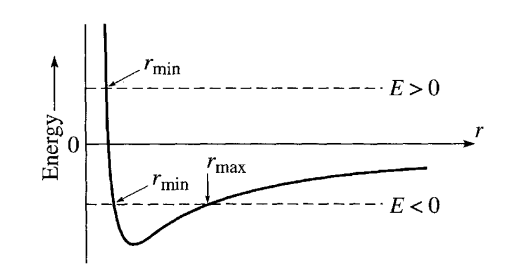
\includegraphics[scale=0.5]{fig1.png}
\end{figure}

First, we consider $E>0$. Looking at figure 1, a comet with this energy can move anywhere such that the line labeled $E>0$ is above the curve of $U_{\text{eff}}(r)$, but nowhere that the line is below the curve. This means that the comet cannot move anywhere inside the turning point labeled $r_min$m determined by the condition
\begin{align*}
  % \label{eq:}
  U_\text{eff}(r_\text{min}) = E.
\end{align*}
If the comet is initially moving in towards the sun, then it will continue until it reaches $r_\text{min}$, where $\dot{r} = 0$ instantaneously. This results in an outwards movement, and since there are no other points where $\dot{r}$ can vanish, the movement of the comet moves off to infinity. Thus, the orbit of the comet is unbounded.

If $E<0$, then the line labeled $E<0$ meets the curve of $U_\text{eff}(r)$ at the two points labeled $r_\text{min}$ and $r_\text{max}$. Thus, the trajectory of the comet is trapped between these two values of r. If it is moving away from the sun, it does so until it reaches $r_\text{max}$, where $\dot{r}$ vanishes and reverses sign. It then moves inward until it reaches $r_\text{min}$, where $\dot{r}$ reverses again. Therefore, the comet oscillates between $r_\text{min}$ and $r_\text{max}$ for all time. This is a bounded orbit.

Finally, although not a central case, if E is exactly equal to the minimum value of $U_\text{eff}(r)$ for a given value of $l$, the two turning points combine, and the comet is trapped at a fixed radius and moves in a circular orbit.




\newpage
\section{Appendix}
\begin{defns}
    \label{def: Configuration Space}
  Consider a system of point masses. 
  \begin{enumerate}
    \item Specifying the position of all the constituent particles of a system specifies the \textbf{configuration} of the system.
    \item The set of all configurations that can be assumed is called the \textbf{configuration space} of the system.
    \item The \textbf{dimension} of the configuration space is the smallest number of parameters needed to completely specify a configuration.
    \item The dimension of the configuration space is called the number of \textbf{degrees of freedom} that a system has.
  \end{enumerate}
\end{defns}

\begin{thebibliography}{9}
\bibitem{1} \label{b1}
        Sussman, G. J. and Mayer, M. E. and Wisdom, J. Structure and Interpretation of Classical Mechanics. MIT Press, Cambridge, 2015. 
\bibitem{2} \label{b2}
        Arnold, V. I. Mathematical Methods of Classical Mechanics, Graduate Texts in Mathematics. Springer, Berlin, 1978.
\bibitem{3} \label{b2}
        Taylor, J. R. Classical Mechanics. University Science Books, 2005.
\bibitem{4} \label{bh}
        Shapiro, J. A. Classical Mechanics. Rutgers University, New Jersey, 2010.
\bibitem{5} \label{b3}
        Kao, C.Z. Classical Mechanics: The Three-Body Problem. University of Chicago, Chicago, 2011.
\bibitem{6} \label{b4}
        Morin, D. Introduction to Classical Mechanics: With Problems and Solutions. Cambridge University Press, Cambridge, 2008.
\bibitem{7} \label{b5}
        Chertkov, M. and Clark, C. Lecture Notes on the Principles and Methods of Applied Mathematics. University of Arizona, Tucson, 2020.
\bibitem{8} \label{b5}
        Singer, S.F. Symmetry in Mechanics: A Gentle, Modern Introduction. Birkhauser, 2004.
\bibitem{9}
        Spivak, M. Physics for Mathematicians, Mechanics I. Publish or Perish Press, 2010. Online Access.
\end{thebibliography}

\end{document}